\documentclass{anstrans}
%%%%%%%%%%%%%%%%%%%%%%%%%%%%%%%%%%%
\title{Adjoint-based Sensitivity for Radiation Transport Using an Eddington Tensor Formulation}
\author{Ian Halvic,$^{*}$ Jean Ragusa,$^{*}$}

\institute{
$^{*}$ Texas A\&M University,
College Station, TX, iwhalvic@tamu.edu}


% Optional disclaimer: remove this command to hide
%\disclaimer{Notice: this manuscript is a work of fiction. Any resemblance to
%actual articles, living or dead, is purely coincidental.}

%%%% packages and definitions (optional)
\usepackage{graphicx} % allows inclusion of graphics
\usepackage{booktabs} % nice rules (thick lines) for tables
\usepackage{microtype} % improves typography for PDF
\usepackage{amsmath, amssymb, amsfonts, float, esint, subcaption, xspace, xcolor, multirow} 
%\newcommand{\SN}{S$_N$}
%\renewcommand{\vec}[1]{\bm{#1}} %vector is bold italic
%\newcommand{\vd}{\bm{\cdot}} % slightly bold vector dot
%\newcommand{\grad}{\vec{\nabla}} % gradient
%\newcommand{\ud}{\mathop{}\!\mathrm{d}} % upright derivative symbol

\newcommand{\vr}{\vec{r}}
\newcommand{\vp}{\vec{p}}
\newcommand{\vOmega}{\vec{\Omega}}
\newcommand{\vJ}{\vec{J}}
\newcommand{\vO}{\vec{\Omega}}
\newcommand{\bra}{\left\langle}
\newcommand{\ket}{\right\rangle}
\newcommand{\braSN}{\left\langle}
\newcommand{\ketSN}{\right\rangle_{\Omega}}
\newcommand{\sbraSN}{\left[ \! \left[}
\newcommand{\sketSN}{\right] \! \right]}
\newcommand{\sbra}{\left[}
\newcommand{\sket}{\right]}
\renewcommand{\div}{\vec{\nabla} \cdot}
\newcommand{\grad}{\vec{\nabla}}
\newcommand{\vbeta}{\vec{\beta} }
\newcommand{\pdx}{\frac{\partial}{\partial x}}
\newcommand{\pdy}{\frac{\partial}{\partial y}}
\newcommand{\pdz}{\frac{\partial}{\partial z}}
\newcommand{\intrrr}{\int d^3 r \,}
\newcommand{\intrr}{\int d^2 r \,}
\newcommand{\dEdphi}{\partial_\phi E }
\newcommand{\dEdp}{\partial_p E }
\newcommand{\dBdphi}{\partial_\phi B }
\newcommand{\dBdp}{B }
\newcommand{\adj}{\phi^\dag}
\newcommand{\vefadj}{\varphi^\dag}
\newcommand{\surf}{\int_{\partial V}}
\newcommand{\domain}{V}
\newcommand{\bound}{\partial V}
\newcommand{\vn}{\vec{n}}
\newcommand{\Edd}{\mathbb{E}}
\newcommand{\BEdd}{B}
\newcommand{\sigt}{\sigma_t}
\newcommand{\sigs}{\sigma_s}
\newcommand{\siga}{\sigma_a}
%\newcommand{\isigt}{\sigma_t^{-1}}
%\newcommand{\isigtp}{\sigma_{t,p}^{-1}}
\newcommand{\isigt}{\ell_t}
\newcommand{\isigtp}{\ell_{t,p}}
\newcommand{\angSource}{\frac{q}{4 \pi}}
\newcommand{\angSourcep}{\frac{q_p}{4 \pi}}
\newcommand{\angSourcepd}{\frac{q_p+\delta q_p}{4 \pi}}
\newcommand{\angSourced}{\frac{\delta q}{4 \pi}}
\newcommand{\scalSource}{q}
\newcommand{\angResp}{q^\dag}
\newcommand{\scalResp}{q^\dag}
\newcommand{\qoi}{{\it QoI}\xspace}


\newcommand{\comment}[2]{\marginpar{\textcolor{#2}{$\star$}}\textcolor{#2}{#1}\newline}

%-----------------------------------------------------------
%-----------------------------------------------------------
\usepackage{ifthen}
\newboolean{draftversion}
\setboolean{draftversion}{false}
%-----------------------------------------------------------
%----------------------------------------------------------

\ifthenelse{\boolean{draftversion}}
{
\newcommand{\iwh}[1]{\comment{#1}{red}}
\newcommand{\jcr}[1]{\comment{#1}{blue}}
\newcommand{\todo}[1]{\comment{#1}{purple}}
}
{
\newcommand{\iwh}[1]{\phantom{a}}
\newcommand{\jcr}[1]{\phantom{a}}
\newcommand{\todo}[1]{\phantom{a}}
}

\newcommand{\tcr}[1]{\textcolor{red}{#1}}

\begin{document}
%%%%%%%%%%%%%%%%%%%%%%%%%%%%%%%%%%%%%%%%%%%%%%%%%%%%%%%%%%%%%%%%%%%%%%%%%%%%%%%%
\section{Introduction}


Adjoint methods are of particular interest for UQ. In general, adjoint methods provide a mechanism for propagating uncertainty and error in the system variables to the uncertainty in the desired quantity of interest (\qoi). This is accomplished in a particularly economical way, sometimes requiring only two differential system solves which can then be used for any combination of sources of error, as opposed to performing an independent solve for each individual error scenario. These adjoint methods have been applied across various complex and time dependent systems. An example of adjoint methods applied to hydrodynamic systems with shocks can be found in Wildey et al. \cite{Wildey}. A more relevant adjoint example to neutron transport occurs in Stripling et al. in the form of reactor burn-up equations \cite{Stripling}.


Application of the adjoint method to transport can pose a major technical limitation. In general, the adjoint method applied to radiation transport requires storing six-dimensional data (the forward angular flux). When dealing with high resolution in these six dimensions, this can potentially require an unreasonable amount of memory for data storage, rendering the method functionally unusable. 

A potential solution to the memory requirement for the transport adjoint formulation is the use of a quasi-diffusion method to reduce the overall dimensionality of the transport problem, from 6D+time to 4D+time. The quasi-diffusion method examined is termed  as a ``Variable Eddington Tensor'' (VET) formulation and uses the unperturbed forward angular flux to compute the Eddington tensor needed in the quasi-diffusion approach. 

In this paper the simpler 1-group steady state problem is considered. Examination of effectiveness of an adjoint formalism using the quasi-diffusion approximation instead of the full transport solution in this setting will provide insight to the advantages and shortcomings of the technique when applied to the multigroup time-dependent problem. If the treatment that is presented here is also applied to the time-dependent one-group system, the Eddington term found in Eq.~\eqref{eqs:sensitivity} also appears. 
%%%%%%%%%%%%%%%%%%%%%%%%%%%%%%%%%%%%%%%%%%%%%%%%%%%%%%%%%%%%%%%%%%%%%%%%%%%%%%%%
\section{Theory}
The notation for inner products used throughout is as follows:
\begin{itemize}
\item $\braSN \psi , f \ketSN  := \int_V dV \int_{4 \pi} d \Omega \,  \psi(\vr, \vO)f(\vr, \vO) \,$

\item $\bra \phi , f \ket : = \int_V dV \,  \phi(\vr) g(\vr) \,$

\item $\sbraSN \psi , f \sketSN_{\pm}   := \int_{\bound} dS \int_{\vO \cdot \vn \gtrless 0} d\Omega \,  \vO \cdot \vn(\vr) \, \psi(\vr, \vO)f(\vr, \vO) \,$

\item $\sbra \phi(\vr) , g(\vr)  \sket := \int_{\partial V} dS \, \phi (\vr) g (\vr)  \,$
\end{itemize}

\subsection{Background}
For this work the \qoi values considered are restricted to those than can be expressed in the form $\qoi := \bra \phi , q^\dag \ket $ where $q^\dag$ is the response function. This definition can handle total and average flux counting as well as simple detector setups.
The one-group steady-state transport system we focus on is defined as
\begin{subequations}
\begin{equation}
\label{SS1GTE}
\vO \cdot \grad \psi + \sigt \psi = \frac{1}{4 \pi} \sigs \phi + \frac{1}{4 \pi} q \in V
\end{equation}
\begin{equation}
\label{eqs:SS1GTE_bc}
\psi= \psi^{\text{inc}} \quad \vr \in \partial V^{-} = \{ \vr \in \bound, \text{ s.t. }, \vO \cdot \vec{n}(\vr) < 0\}.
\end{equation}
\end{subequations}
In addition to the forward transport system, the appropriate adjoint transport system for the \qoi definition in use is 
\begin{subequations}
\begin{equation}
\label{eqs:transAdj}
- \vO \cdot \grad \psi^\dag + \sigt \psi^\dag = \frac{\sigs}{4 \pi} \phi^\dag + \scalResp
\end{equation}
\begin{equation}
\psi^\dag =0 \quad \vr \in \partial V^{+} = \{  \vr \in \bound , \text{ s.t. }, \quad \vO \cdot \vec{n} > 0 \}.
\end{equation}
\end{subequations}
The $\delta \qoi$ inner-product for use with one-group adjoint transport is given by Eq.~\eqref{eqs:snSens} \cite{Greenspan}. This formulation utilizes both the scalar and angular fluxes of both the forward and adjoint transport solutions. The requirement to store the angular flux solution for use in the $\delta \sigt$ term is what this research aims to eliminate.

\begin{equation}
\label{eqs:snSens}
\begin{split}
\delta QoI = \bra \angSourced  + \frac{\delta\sigs}{4 \pi} \phi , \phi^\dag  \ket - \braSN  \delta \sigt \psi , \psi^\dag \ketSN - \sbraSN \delta \psi^{\text{inc}}, \psi^\dag \sketSN_- \,
\end{split}
\end{equation}

\subsection{Eddington Formulation and Sensitivity}

In an effort to circumvent the excessive storage requirement for the angular flux, a quasi-diffusive adjoint approach is considered. The approach relies on the Eddington Tensor ($\Edd$) defined as $\Edd \phi = \int d\Omega \vO \vO \psi$ and a Boundary Eddington Factor $B \phi = \int d\Omega \, | \vO \cdot \vn | \psi$ to generate the quasi-diffusive system. For the one group steady-state case the system is defined as 
\begin{subequations} \label{eqs:EddingtonSystem}
\begin{equation} \label{eq:EddingtonVol}
- \div \left( \isigt \div \Edd \phi \right) + \siga \phi = \scalSource \,,
\end{equation}
inside $\vec{r} \in V$, with boundary condition
\begin{equation} \label{eq:EddingtonBC}
2 J^{\text{inc}} = \BEdd \phi + \vn \cdot \isigt \div \Edd \phi  \quad \vr \in \bound \,,
\end{equation}
\end{subequations}
where $\isigt$ denotes the mean free path $\sigt^{-1}$ \cite{Goldin} \cite{Miften}. Given the correct value of $\Edd$ from an initial transport solve, the Eddington System can exactly compute the scalar flux $\phi$, which is sufficient for obtaining quantities of interest in the inner product form $\bra q^\dag , \phi \ket$.

The adjoint system of Eq.~\eqref{eqs:EddingtonSystem} relevant for our \qoi definition is given as
\begin{subequations}\label{eqs:EddingtonAdjSystem}
\begin{equation}\label{eq:EddingtonAdjVol}
- \Edd : \grad \left( \isigt \grad \vefadj \right)  + \siga \vefadj = \scalResp
\end{equation}
\begin{equation}\label{eq:EddingtonAdjBC}
0 = B \vefadj+ \vn \cdot
\Edd \cdot \isigt \vec{\nabla} \vefadj    \quad \vr \in \bound .
\end{equation}
\end{subequations}
Solving Eq.~\eqref{eqs:EddingtonAdjSystem} results in a VET adjoint flux $\varphi^\dag$ that is distinctly different from the adjoint flux of the transport formulation ($\phi^\dag \neq \varphi^\dag$). For clarification of the notation used, the adjoint system equation contains a double gradient tensor $(\grad \grad u)_{ij} = \partial_{x_i} \partial_{x_j} u$ along with a tensor dot product $\mathbb{A} : \mathbb{B} = \sum_i \sum_j A_{ij}B_{ij}$.

Perturbations are then introduced in the form of $\delta q$, $\delta \siga$, $\delta \sigt$, and $\delta J^{\text{inc}}$ to generate a perturbed system leading to a change in the desired \qoi. Using a first-order perturbation method and making the assumption that $\Edd$ remains unperturbed, the change in the \qoi can be approximated using the inner product
\begin{equation}\label{eqs:sensitivity}
\delta \qoi =  \bra \delta \scalSource - \delta \siga \phi, \vefadj \ket  - \bra \delta \isigt \div \left( \Edd \phi \right) , \grad \vefadj \ket
 + \sbra \vefadj, 2 \delta J^{\text{inc}} \sket \,.
\end{equation}
This proposed method requires an initial solve of the angular transport system to compute $\phi$ and $\Edd$, which are stored for use in Eq.~\eqref{eqs:sensitivity}, as opposed to storing $\phi$ and $\psi$. For computational transport solution schemes which finely descritize $\Omega$, the VET method should hold a clear advantage in terms of required memory. 

Refinements to the VET method are also considered. The first is relatively low cost ``blended'' method which utilizes both the VET and transport adjoint formulations. This approach selects the most advantageous term for each perturbation from either Eq.~\eqref{eqs:snSens} or Eq.~\eqref{eqs:sensitivity}.  
\begin{equation}
\label{eqs:Blendsens}
\begin{split}
\delta \qoi =&  \bra \angSourced , \phi^\dag \ket - \bra \delta \siga \phi, \vefadj \ket - \bra \delta \isigt \div \left( \Edd \phi \right) , \grad \vefadj \ket\\
&\quad - \sbraSN \delta \psi^\text{inc}, \psi^\dag \sketSN \\
\end{split}
\end{equation}
In the blended form expressed in Eq.~\eqref{eqs:Blendsens} the response to source perturbations are computed using the inner-product terms from the transport adjoint method, which do not require a first order approximation to formulate. Meanwhile the response due to cross-section perturbations are computed using terms from the VET adjoint formulation, which do not require $\psi$ to be stored. The cost of utilizing this method is an additional transport adjoint solve for $\phi^\dag$ when compared to the VET treatment.


A second refinement considered is a method of approximating the Eddington perturbation $\delta \Edd$, which relaxes the unperturbed Eddington assumption required for Eq.~\eqref{eqs:sensitivity}. For scenarios where many perturbation cases are to be considered, utilizing a small amount of additional forward transport solves to characterize the behavior of $\Edd$ under selected perturbations can offer a refinement of the VET method. A simple linear approximation scheme is tested, in which the parameter of interest $p$ is perturbed by $\delta p$ and a slope of $\Edd$ is approximated using an additional transport solve. 
\begin{equation}
\label{Eddapprox}
\frac{\partial \Edd}{\partial p} \approx \frac{\Edd(p+\delta p) - \Edd(p)}{\delta p}
\end{equation}
With $\frac{\partial \Edd}{\partial p}$ known a $\delta \Edd$ can then be approximated for a given perturbation $\delta p$. An analogous method can be used to approximate a $\delta \BEdd$ if desired. The VET sensitivity inner product Eq.~\eqref{eqs:sensitivity} can then be augmented with $\delta \Edd$ and $\delta \BEdd$ terms to improve accuracy
\begin{equation}
\label{eqs:EddErr}
\begin{split}
\delta \qoi &=  \bra \delta \scalSource - \delta \siga \phi, \vefadj \ket  - \bra \delta \isigt \div \left( \Edd \phi \right) , \grad \vefadj \ket
 + \sbra \vefadj, 2 \delta J^{\text{inc}} \sket \\
 & \quad - \bra  \isigt \div \left( \delta \Edd \phi \right), \grad \vefadj \ket
- \sbra \vefadj, \delta \BEdd \phi \sket \,.
\end{split}
\end{equation} 
A particular weakness of this approach is that additional forward solves and Eddington stores are required to characterize $\Edd$ in the the perturbation space, which scales with the number of perturbed variables considered. Therefore in this approach it may be advantageous to only consider perturbations that would have a significant effect of the $\delta \Edd$ or $\delta \BEdd$ terms in Eq.~\eqref{eqs:EddErr} if possible. 


%%%%%%%%%%%%%%%%%%%%%%%%%%%%%%%%%%%%%%%%%%%%%%%%%%%%%%%%%%%%%%%%%%%%%%%%%%%%%%%%
\section{Results}
The approximation of $\delta \qoi$ of various system perturbations using the VET method were tested against the $\delta \qoi$ value found using a transport adjoint method. A reference $\delta \qoi$ value for comparison was found using the difference of two forward transport solves. The VET system was discretized using a discontinuous finite element method with interior penalty \cite{Arnold}. The transport system was discretized using linear discontinuous elements and a discrete ordinates ($S_n$) solver with $n=8$. Both methods utilized the same $2000$ element spacial mesh. Void regions were modeled using a $\sigt=10^{-8}$ value as the existence of the $\isigt$ term in the VET formulations prevent the use of $\sigt=0$.

A test case examined is a 1-dimensional 5 section Reed system \cite{ReedProb}, with forward scalar flux solution show in Figure~\ref{fig:Flux4}. The system is defined on  $x \in [0,8]$ as follows:
\begin{itemize}
\item Region 1: $x \in [0,2), \quad \siga=50, \, 			\sigs=0, \, q=50$
\item Region 2: $x \in [2,3), \quad \siga=5, \, 			\sigs=0, \, q=0$
\item Region 3: $x \in [3,5), \quad \siga=10^{-8} \,	\sigs=0, \, q=0$
\item Region 4: $x \in [5,6), \quad \siga=0.1, \, 		\sigs=0.9, \, q=1$
\item Region 5: $x \in [6,8], \quad \siga=0.1, \, 		\sigs=0.9, \, q=0$
\end{itemize}
 Two $\qoi$ values of the system were considered for comparison, with the resulting adjoint fluxes $\phi^\dag$ and $\varphi^\dag$ presented in Figure~\ref{fig:adj}.
 
 \begin{itemize}
\item $\qoi_5 =1/2 \int_6^8 \phi dx $: The average flux in the scattering Region 5

\item $\qoi_3 =1/2 \int_3^5 \phi dx $: The average flux in the central void Region 3
 \end{itemize}

Table~\ref{tab:qoi1} and Table~\ref{tab:qoi2} present the $\delta \qoi$ values found using the VET inner product given in Eq.~\eqref{eqs:sensitivity} and the two refinement methods mentioned. For VET methods both the absolute $\delta \qoi$ values as well as relative deviation from the transport adjoint $ 100*\left| \delta \qoi_{VET} - \delta \qoi_{Tran}\right|/ \delta \qoi_{Tran}$ are presented.



\begin{figure}[h]
\centering
2 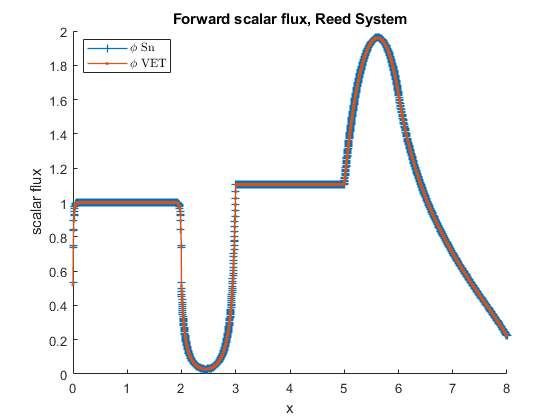
\includegraphics[scale=0.5]{7phi.png}
 \caption{Plot of unperturbed forward scalar flux for the Reed's problem. Flux found using both transport and VET method.}
\label{fig:Flux4}
\end{figure}


\begin{figure}[h]
\centering
\begin{subfigure}{.25\textwidth}
  \centering
  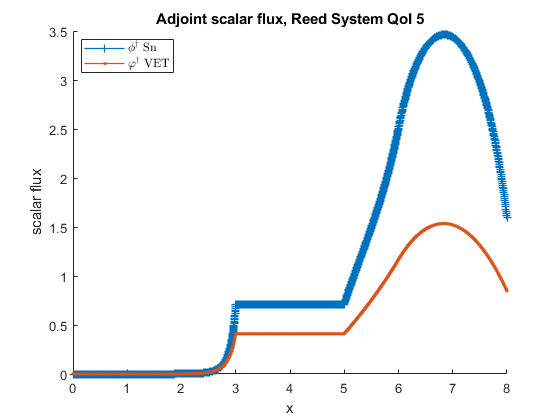
\includegraphics[width=.98\linewidth]{774phia.png}
\end{subfigure}%
\begin{subfigure}{.25\textwidth}
  \centering
  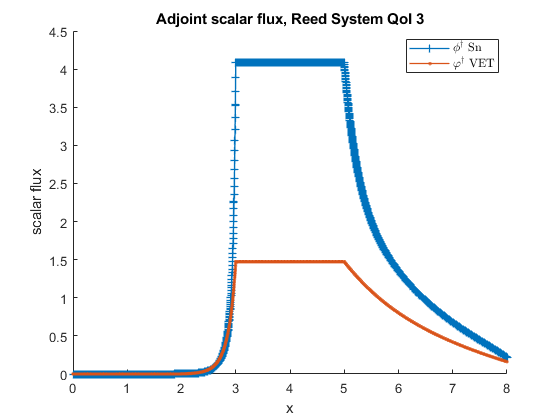
\includegraphics[width=.98\linewidth]{772phia.png}
\end{subfigure}
\caption{Adjoint flux solutions for $\qoi_5$ (left) and $\qoi_3$ (right). For each $\qoi$ considered there is a transport adjoint flux $\phi^\dag$ for use with Eqs.~\eqref{eqs:snSens},~\eqref{eqs:Blendsens}; as well as a VET adjoint flux $\varphi^\dag$ for use with Eq.~\eqref{eqs:sensitivity},~\eqref{eqs:Blendsens},~\eqref{eqs:EddErr}.}
\label{fig:adj}
\end{figure}

\begin{table*}
  \centering
  \caption{$\delta \qoi$ values for $\qoi$ region in scattering material far from voids. ($\%$) values are relative to transport adjoint found values.}
  \begin{tabular}{l|rr|rrr}\toprule
  System Perturbation    & Reference     & Trans adj     & VET adj \hspace{1mm} (\%)    &   VET blended \hspace{1mm} (\%)   & VET $\delta \Edd$-appx  \hspace{1mm} (\%) 
\\ \midrule
$q+10\%$  & 0.0766  & 0.0766  & 0.0765 \hspace{1mm} (0.03 \%)  & 0.0766   \hspace{1mm} (0 \%) & 0.0765787  \hspace{1mm} (0.03 \%)
\\
$\siga+10\%$  &-0.0128  & -0.0130 & -0.0130   \hspace{1mm} (0.28 \%) & -0.0130  \hspace{1mm} (0.28 \%) & -0.0129986  \hspace{1mm} (0.04 \%) 
\\
$\sigs+10\%$  & 0.00856  & 0.00852  & 0.00683  \hspace{1mm} (19.87 \%)  & 0.00683   \hspace{1mm} (19.87 \%) & 0.00768   \hspace{1mm} (9.89 \%)
\\
$q+10\%,\siga+10\%$  & 0.0625 & 0.0636  & 0.0635 \hspace{1mm} (0.09 \%) & 0.0636 \hspace{1mm} (0.06 \%)  &  0.0636  \hspace{1mm} (0.03 \%)
\\
\bottomrule
\end{tabular}
  \label{tab:qoi1}
\end{table*}


\begin{table*}
  \centering
  \caption{$\delta \qoi$ values for $\qoi$ region within void. ($\%$) values are relative to transport adjoint found values.}
  \begin{tabular}{l|rr|rrr}\toprule
  System Perturbation    & Reference     & Trans adj     & VET adj \hspace{1mm} (\%)    &   VET blended \hspace{1mm} (\%)   & VET $\delta \Edd$-appx  \hspace{1mm} (\%) 
\\ \midrule
$q+10\%$  & 0.111   & 0.111   & 0.110 \hspace{1mm} (0.07 \%) & 0.111   \hspace{1mm} (0 \%) & 0.110 \hspace{1mm} (0.07 \%) 
\\
$\siga+10\%$  &-0.0207  & -0.0210 & -0.0203  \hspace{1mm} (3.60 \%)  & -0.0203 \hspace{1mm} (3.60 \%)  & -0.0210 \hspace{1mm} ( 0.20 \%) 
\\
$\siga+10\%$  & -0.00953   & -0.00992   & 0.00135   \hspace{1mm} (113.65 \%)  & 0.00135  \hspace{1mm} (113.65 \%)  & -0.00950 \hspace{1mm} (4.19 \%) 
\\
$q+10\%,\siga+10\%$  & 0.0878  & 0.0895  & 0.0901 \hspace{1mm} (0.76 \%)  & 0.0902 \hspace{1mm} (0.85 \%)   &  0.0894   \hspace{1mm} (0.04 \%) 
\\
\bottomrule
\end{tabular}
  \label{tab:qoi2}
\end{table*}


In addition to the two $\qoi$ cases presented in this summary, additional $\qoi$ regions of the above system are also examined in a similar manner in the full work. Beyond the Reed system presented here additional systems were also tested in the full work, including a simple shielding system to demonstrate the effect of an perturbation in the incident flux $\delta \psi^{inc}$ and incident current $\delta J^{inc}$.



%%%%%%%%%%%%%%%%%%%%%%%%%%%%%%%%%%%%%%%%%%%%%%%%%%%%%%%%%%%%%%%%%%%%%%%%%%%%%%%%
\section{Conclusions}
For both test systems under source perturbation, all VET methods perform to within 1\% of the transport adjoint method. As constructed, the blended method inherits the transport adjoint's ability to return the reference value due to no first-order approximation. The $\qoi_5$ system performs somewhat better for absorption cross-section perturbations compared to the $\qoi_3$ system, though even in the worse performing system the discrepancy is under 5\%. Utilization of the $\delta \Edd$ further reduces the discrepancy in both systems. The $\delta \qoi$ results of the scenario in which both the source and the absorption cross-section are perturbed tends to follow the behavior of the source perturbation scenario, primarily due to the larger magnitude of the source perturbation response. 

Perturbations in the scattering cross-sections show the strongest deviation of  the VET method from transport adjoint. For the $\qoi_3$ test the VET adjoint method and the blended are functionally useless. However, using an additional transport solve to begin to characterize the $\delta \Edd$ value had a drastic effect in this scenario and results in a much more usable value. One possible explanation is that in Eq.~\eqref{eqs:EddErr} the $\delta \Edd$ term is multiplied by a factor of $\isigt$. With the $\qoi$ region on the boundary of a void there is a significant numerical contribution from this $\isigt$ value, which resolves to a very large number in for the numerical scheme chosen. This gives some evidence that when using the $\delta \Edd$ approximation method it may be advantageous to characterize the $\Edd$ behavior under perturbation at void boundaries near a selected $\qoi$ region.

An aspect of future work will focus on refinement of the solution method for dealing with void regions, perhaps employing more elegant methods than the small cross-section approximation used in this implementation.

%%%%%%%%%%%%%%%%%%%%%%%%%%%%%%%%%%%%%%%%%%%%%%%%%%%%%%%%%%%%%%%%%%%%%%%%%%%%%%%%
\appendix
%\section{Appendix}

%Inner-products used
%\begin{equation}
%\braSN \psi , f \ketSN  = \int_V dV \int_{4 \pi} d \Omega \,  \psi(\vr, \vO)f(\vr, \vO) \,
%\end{equation}
%\begin{equation}
%\sbraSN \psi , f \sketSN_{\pm}   = \int_{\bound} dS \int_{\vO \cdot \vn \gtrless 0} d\Omega \,  \vO \cdot \vn(\vr) \, \psi(\vr, \vO)f(\vr, \vO) \,
%\end{equation}
%\begin{equation}
%\bra \phi(\vr) , f \ket  = \int_V dV \,  \phi(\vr) g(\vr) \,
%\end{equation}
%\begin{equation}
%\sbra \phi(\vr) , g(\vr)  \sket = \int_{\partial V} dS \, \phi (\vr) g (\vr)  \,
%\end{equation}
%
%\begin{subequations}\label{eqs:TransportSystem}
%\begin{equation}
%\label{SS1GTE}
%\vO \cdot \grad \psi(\vr,\vO) + \sigt(\vr) \psi(\vr,\vO) = \frac{1}{4 \pi} \sigs(\vr) \phi(\vr) + \frac{1}{4 \pi} q(\vr)\, ,
%\end{equation}
%\begin{equation}
%\label{SS1GTE_bc}
%\psi(\vr,\vO) = \psi^{\text{inc}}(\vr,\vO) \quad \vr \in \partial V^{-} = \{ \vr \in \partial V,  \vO \cdot \vec{n}(\vr) < 0\}
%\end{equation}
%\end{subequations}
%\begin{subequations}\label{eqs:TransportAdjSystem}
%\begin{equation}
%\label{SS1GTE}
%- \vO \cdot \grad \psi^\dag(\vr,\vO) + \sigt(\vr) \psi^\dag(\vr,\vO) = \frac{1}{4 \pi} \sigs(\vr) \phi^\dag(\vr) + q^\dag(\vr)\, ,
%\end{equation}
%\begin{equation}
%\label{SS1GTE_bc}
%\psi^\dag(\vr,\vO) = \psi^{\dag,\text{out}}(\vr,\vO) \quad \vr \in \partial V^{+} = \{ \vr \in \partial V,  \vO \cdot \vec{n}(\vr) > 0\}
%\end{equation}
%\end{subequations}
%Sensitivity
%\begin{equation}
%\delta \qoi = \bra \angSourced  + \frac{\delta\sigs}{4 \pi} \phi , \phi^\dag  \ket - \braSN  \delta \sigt \psi , \psi^\dag \ketSN - \sbraSN \delta \psi^{\text{inc}}, \psi^\dag \sketSN_- \,.
%\end{equation}

%%%%%%%%%%%%%%%%%%%%%%%%%%%%%%%%%%%%%%%%%%%%%%%%%%%%%%%%%%%%%%%%%%%%%%%%%%%%%%%%
\section{Acknowledgments}
The work presented was supported by a graduate assistantship from the U.S. DOE NNSA's PSAAP program (Predictive Science Academic Alliance Program), Grant DE-NA0002376.  

%%%%%%%%%%%%%%%%%%%%%%%%%%%%%%%%%%%%%%%%%%%%%%%%%%%%%%%%%%%%%%%%%%%%%%%%%%%%%%%%
\bibliographystyle{ans}
\bibliography{QoI_MS}
\end{document}

